\section{Análise dos Dados}\label{sec:analise-dos-dados}

\begin{frame}{Análise dos Dados}
	\begin{block}{}
		\begin{itemize}
			\item Essencial para determinar o sucesso do estudo;
			\item Médias dos quatro testes realizados (10\%, 20\%, 40\%, 80\%)
			\item Comparação através de gráficos e dados;
			\item Por faixas de requisições e todas as requisições.
		\end{itemize}
	\end{block}
\end{frame}

\begin{frame}{Organização dos gráficos e dados}
	\begin{block}{Faixas}
		\begin{itemize}
			\item \textbf{Faixa 1} - Entre 1.000 e 5.000 requisições totais;
			\item \textbf{Faixa 2} - Entre 6.000 e 10.000 requisições totais;
			\item \textbf{Faixa 3} - Entre 11.000 e 15.000 requisições totais.
		\end{itemize}
	\end{block}
\end{frame}

\begin{frame}{Média do Tempo Total de Execução dos Testes}
	\begin{figure}
		\centering
		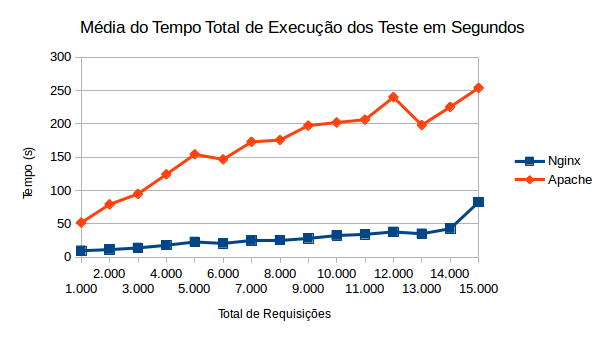
\includegraphics[width=1\linewidth]{../graficos/grafico1} 
	\end{figure}
\end{frame}

\begin{frame}{Média do Total de Dados Transferido}
	\begin{figure}
		\centering
		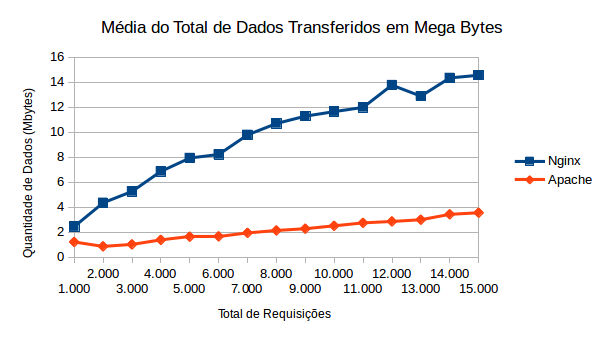
\includegraphics[width=1\linewidth]{../graficos/grafico2} 
	\end{figure}
\end{frame}

\begin{frame}{Média do Total de Texto HTML Transferido}
	\begin{figure}
		\centering
		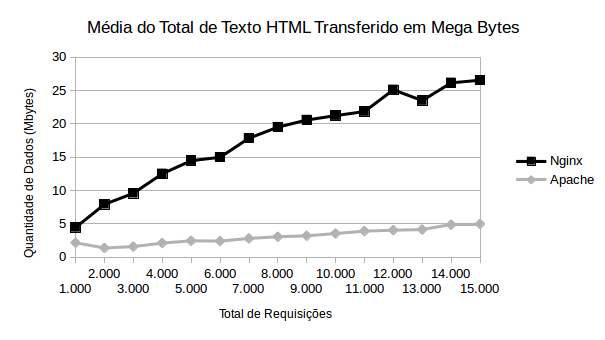
\includegraphics[width=1\linewidth]{../graficos/grafico3} 
	\end{figure}
\end{frame}

\begin{frame}{Média do Número de Requisições Atendidas}
	\begin{figure}
		\centering
		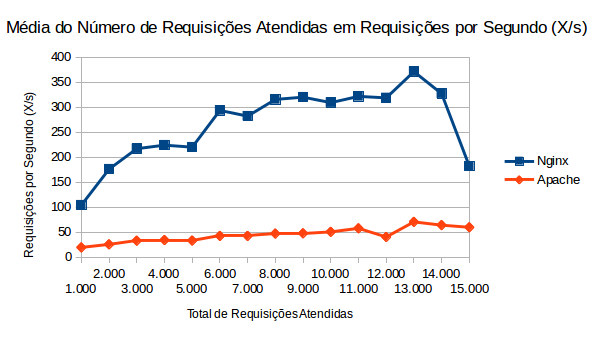
\includegraphics[width=1\linewidth]{../graficos/grafico4} 
	\end{figure}
\end{frame}

\begin{frame}{Média do Tempo de Resposta por Requisição Simultânea}
	\begin{figure}
		\centering
		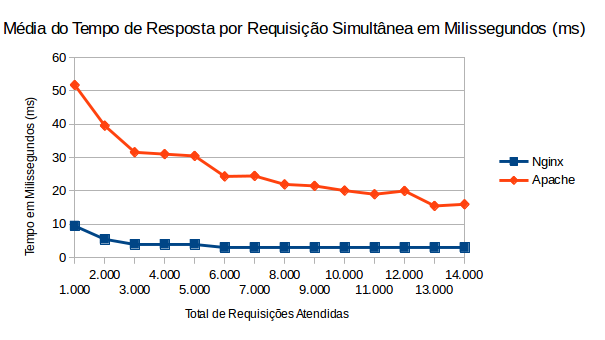
\includegraphics[width=1\linewidth]{../graficos/grafico5} 
	\end{figure}
\end{frame}

\begin{frame}{Média da Taxa de Transferência}
	\begin{figure}
		\centering
		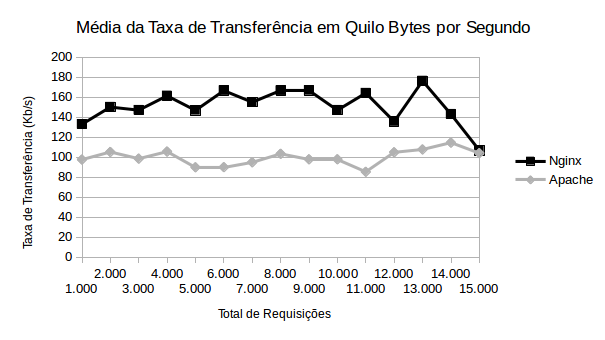
\includegraphics[width=1\linewidth]{../graficos/grafico6} 
	\end{figure}
\end{frame}

